\documentclass{beamer}
\usepackage{graphicx} % Required for inserting images
\usetheme{Madrid}
\usepackage{tikz}
\usetikzlibrary{arrows}
\usepackage{amsthm}
\usepackage[utf8]{inputenc}
\usepackage[usenames,dvipsnames]{xcolor}
\usepackage[upright]{fourier}
\usepackage{tkz-graph}
\usetikzlibrary{arrows}
\title{Travelling Salesman Problem}
\author[Nayem \and Jayed \and Iffat]{M.M. Nayem\inst{1} \and Kazi Jayed Haider\inst{2} \and Iffat Bin Hossain\inst{3}}
\date{\today}
\institute[VFU] % (optional)
{
  \inst{1}%
  2005078\\
  \and
  \inst{2}%
  2005081\\
\and
\inst{3}%
2005087\\
  
}

\begin{document}
\maketitle
\begin{frame}
\frametitle{Table of Contents}
\tableofcontents
\end{frame}

% Nayem's Part started

\begin{frame}{Introduction}
\section{Introduction}
\newtheorem{What is TSP?}{What is TSP?}
\begin{What is TSP?}
\textbf{Travelling salesman problem (TSP)}, asks the following question: "Given a list of cities and the distances between each pair of cities, what is the shortest possible route that visits each city exactly once and returns to the origin city?" \cite{tsp-wikipedia}
\end{What is TSP?}
\end{frame}

\begin{frame}
  \begin{figure}[h]
    \centering
    \includegraphics[scale=0.3]{TSP.jpg}
    \caption{TSP}
    \label{fig:enter-label}
\end{figure}  
\end{frame}
\section{Why TSP is Interesting?}
\begin{frame}{Why TSP is Interesting?}
    \begin{itemize}
        \item It's NP-hard problem in complexity theory
         \item Algorithmic Challenges
         \item Benchmark Problem
         \item Real-world Applications
    \end{itemize}
\end{frame}
\section{Real-world Applications}
\begin{frame}{Real-world Applications}
    \begin{figure}
        \centering
        \includegraphics[scale=0.4]{photo_2024-02-20_04-05-08.jpg}
        \caption{In Hubble Telescope}
        \label{fig:enter-label}
    \end{figure}
\end{frame}
\section{Why TSP can't be solved using Greedy Algothim?}
\begin{frame}{Why TSP can't be solved using Greedy?}
\begin{itemize}
    \item Can be proved Mathematically That TSP can't be solved using Greedy approach
\end{itemize}
\begin{examples}
Consider a complete graph with 4 vertices A(0,0),B(0,1),C(2,0),D(3,1)
A Salesman starts in A,here B is 1 unit away,C is 2 unit away,D is 3.16 unit away
The salesman goes to B which is closest,then C is 2.24 unit away and D is 3 away
The salesman goes to C which is closest,then to D which is the last unvisited city then back to A . The total trip A-B-C-D-A is 7.81 long,while the trip A-B-D-C-A is 7.41 unit long.Thus Greedy fails.
\end{examples}
\end{frame}  
\begin{frame}{Why TSP can't be solved using Greedy}
\centering
        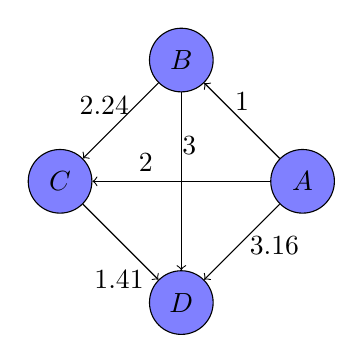
\begin{tikzpicture}[scale=0.22]
    \tikzset{vertex/.style = {shape=circle, draw, fill=blue!50, minimum size=2.3 em}}
    \tikzset{edge/.style = {draw=green, ultra thick, -}}

    % vertices
    \node[vertex] (b) at  (7,0) {$A$};
    \node[vertex] (c) at  (0,7) {$B$};
    \node[vertex] (d) at  (-7,0){$C$};
    \node[vertex] (e) at  (0,-7){$D$};

    % edges
    \draw [->] (b) -- node[pos = 0.8, above,xshift = 7mm]{3.16} (e);
    \draw [->] (b) -- node[midway, above]{1} (c);
    \draw [->] (b) -- node[pos=0.7,above]{2} (d);
    \draw [->] (c) -- node[pos= 0.3pt,xshift = 1mm]{3} (e);
    \draw [->] (c) -- node[pos= 0.3pt,xshift = -4mm]{2.24} (d);
    \draw [->] (d) -- node[pos=1, xshift = -5mm]{1.41} (e);
\end{tikzpicture}
    \begin{examples}
Consider a complete graph with 4 vertices A(0,0),B(0,1),C(2,0),D(3,1)
A Salesman starts in A,here B is 1 unit away,C is 2 unit away,D is 3.16 unit away
The salesman goes to B which is closest,then C is 2.24 unit away and D is 3 away
The salesman goes to C which is closest,then to D which is the last unvisited city then back to A . The total trip A-B-C-D-A is 7.81 long,while the trip A-B-D-C-A is 7.41 unit long.Thus Greedy fails.
\end{examples}
\end{frame}

\begin{frame}{Why TSP can't be solved using Greedy}
\centering
        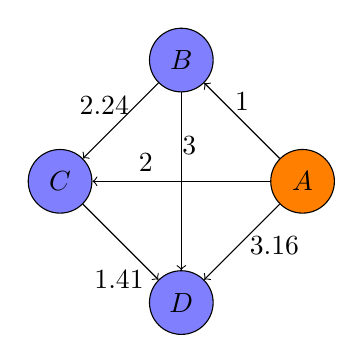
\begin{tikzpicture}[scale=0.22]
    \tikzset{vertex/.style = {shape=circle, draw, fill=blue!50, minimum size=2.3em}}
    \tikzset{edge/.style = {draw=green, ultra thick, -}}

    % vertices
    \node[vertex, fill=orange!100] (b) at  (7,0) {$A$};
    \node[vertex] (c) at  (0,7) {$B$};
    \node[vertex] (d) at  (-7,0){$C$};
    \node[vertex] (e) at  (0,-7){$D$};

    % edges
    \draw [->] (b) -- node[pos = 0.8, above,xshift = 7mm]{3.16} (e);
    \draw [->] (b) -- node[midway, above]{1} (c);
    \draw [->] (b) -- node[pos=0.7,above]{2} (d);
    \draw [->] (c) -- node[pos= 0.3pt,xshift = 1mm]{3} (e);
    \draw [->] (c) -- node[pos= 0.3pt,xshift = -4mm]{2.24} (d);
    \draw [->] (d) -- node[pos=1, xshift = -5mm]{1.41} (e);
\end{tikzpicture}
\begin{examples}
Consider a complete graph with 4 vertices A(0,0),B(0,1),C(2,0),D(3,1)
A Salesman starts in A,here B is 1 unit away,C is 2 unit away,D is 3.16 unit away
The salesman goes to B which is closest,then C is 2.24 unit away and D is 3 away
The salesman goes to C which is closest,then to D which is the last unvisited city then back to A . The total trip A-B-C-D-A is 7.81 long,while the trip A-B-D-C-A is 7.41 unit long.Thus Greedy fails.
\end{examples}
\end{frame}   
\begin{frame}{Why TSP can't be solved using Greedy}
\centering
        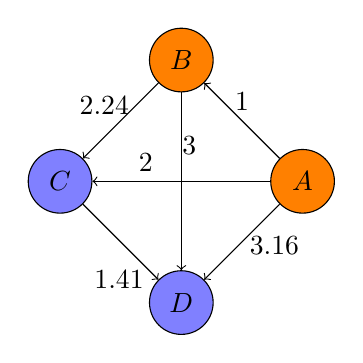
\begin{tikzpicture}[scale=0.22]
    \tikzset{vertex/.style = {shape=circle, draw, fill=blue!50, minimum size=2.3em}}
    \tikzset{edge/.style = {draw=green, ultra thick, -}}

    % vertices
    \node[vertex, fill=orange!100] (b) at  (7,0) {$A$};
    \node[vertex, fill=orange!100] (c) at  (0,7) {$B$};
    \node[vertex] (d) at  (-7,0){$C$};
    \node[vertex] (e) at  (0,-7){$D$};

    % edges
    \draw [->] (b) -- node[pos = 0.8, above,xshift = 7mm]{3.16} (e);
    \draw [->] (b) -- node[midway, above]{1} (c);
    \draw [->] (b) -- node[pos=0.7,above]{2} (d);
    \draw [->] (c) -- node[pos= 0.3pt,xshift = 1mm]{3} (e);
    \draw [->] (c) -- node[pos= 0.3pt,xshift = -4mm]{2.24} (d);
    \draw [->] (d) -- node[pos=1, xshift = -5mm]{1.41} (e);
    
    
    
    
    
\end{tikzpicture}
\begin{examples}
Consider a complete graph with 4 vertices A(0,0),B(0,1),C(2,0),D(3,1)
A Salesman starts in A,here B is 1 unit away,C is 2 unit away,D is 3.16 unit away
The salesman goes to B which is closest,then C is 2.24 unit away and D is 3 away
The salesman goes to C which is closest,then to D which is the last unvisited city then back to A . The total trip A-B-C-D-A is 7.81 long,while the trip A-B-D-C-A is 7.41 unit long.Thus Greedy fails.
\end{examples}
\end{frame}
\begin{frame}{Why TSP can't be solved using Greedy}
\centering
        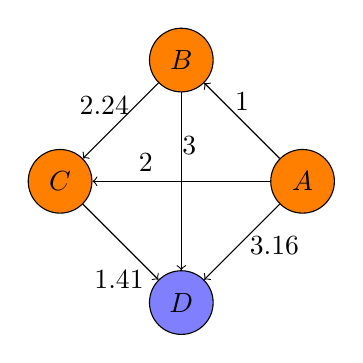
\begin{tikzpicture}[scale=0.22]
    \tikzset{vertex/.style = {shape=circle, draw, fill=blue!50, minimum size=2.3em}}
    \tikzset{edge/.style = {draw=green, ultra thick, -}}

    % vertices
    \node[vertex, fill=orange!100] (b) at  (7,0) {$A$};
    \node[vertex, fill=orange!100] (c) at  (0,7) {$B$};
    \node[vertex, fill=orange!100] (d) at  (-7,0){$C$};
    \node[vertex] (e) at  (0,-7){$D$};

    % edges
    \draw [->] (b) -- node[pos = 0.8, above,xshift = 7mm]{3.16} (e);
    \draw [->] (b) -- node[midway, above]{1} (c);
    \draw [->] (b) -- node[pos=0.7,above]{2} (d);
    \draw [->] (c) -- node[pos= 0.3pt,xshift = 1mm]{3} (e);
    \draw [->] (c) -- node[pos= 0.3pt,xshift = -4mm]{2.24} (d);
    \draw [->] (d) -- node[pos=1, xshift = -5mm]{1.41} (e);
\end{tikzpicture}
\begin{examples}
Consider a complete graph with 4 vertices A(0,0),B(0,1),C(2,0),D(3,1)
A Salesman starts in A,here B is 1 unit away,C is 2 unit away,D is 3.16 unit away
The salesman goes to B which is closest,then C is 2.24 unit away and D is 3 away
The salesman goes to C which is closest,then to D which is the last unvisited city then back to A . The total trip A-B-C-D-A is 7.81 long,while the trip A-B-D-C-A is 7.41 unit long.Thus Greedy fails.
\end{examples}
\end{frame}
\begin{frame}{Why TSP can't be solved using Greedy}
\centering
        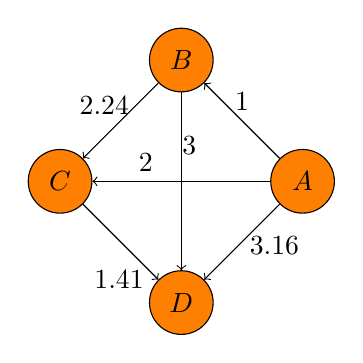
\begin{tikzpicture}[scale=0.22]
    \tikzset{vertex/.style = {shape=circle, draw, fill=blue!50, minimum size=2.3em}}
    \tikzset{edge/.style = {draw=green, ultra thick, -}}

    % vertices
    \node[vertex, fill=orange!100] (b) at  (7,0) {$A$};
    \node[vertex, fill=orange!100] (c) at  (0,7) {$B$};
    \node[vertex, fill=orange!100] (d) at  (-7,0){$C$};
    \node[vertex, fill=orange!100] (e) at  (0,-7){$D$};

    % edges
    \draw [->] (b) -- node[pos = 0.8, above,xshift = 7mm]{3.16} (e);
    \draw [->] (b) -- node[midway, above]{1} (c);
    \draw [->] (b) -- node[pos=0.7,above]{2} (d);
    \draw [->] (c) -- node[pos= 0.3pt,xshift = 1mm]{3} (e);
    \draw [->] (c) -- node[pos= 0.3pt,xshift = -4mm]{2.24} (d);
    \draw [->] (d) -- node[pos=1, xshift = -5mm]{1.41} (e);
\end{tikzpicture}
\begin{examples}
Consider a complete graph with 4 vertices A(0,0),B(0,1),C(2,0),D(3,1)
A Salesman starts in A,here B is 1 unit away,C is 2 unit away,D is 3.16 unit away
The salesman goes to B which is closest,then C is 2.24 unit away and D is 3 away
The salesman goes to C which is closest,then to D which is the last unvisited city then back to A . The total trip A-B-C-D-A is 7.81 long,while the trip A-B-D-C-A is 7.41 unit long.Thus Greedy fails.
\end{examples}
\end{frame}
\begin{frame}{Why TSP can't be solved using Greedy}
\centering
        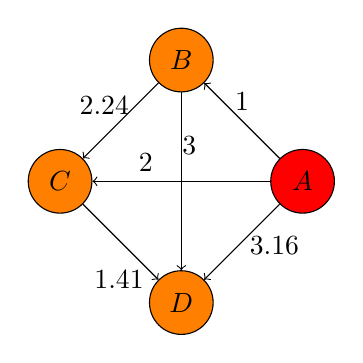
\begin{tikzpicture}[scale=0.22]
    \tikzset{vertex/.style = {shape=circle, draw, fill=blue!50, minimum size=2.3em}}
    \tikzset{edge/.style = {draw=green, ultra thick, -}}

    % vertices
    \node[vertex, fill=red!100] (b) at  (7,0) {$A$};
    \node[vertex, fill=orange!100] (c) at  (0,7) {$B$};
    \node[vertex, fill=orange!100] (d) at  (-7,0){$C$};
    \node[vertex, fill=orange!100] (e) at  (0,-7){$D$};

    % edges
    \draw [->] (b) -- node[pos = 0.8, above,xshift = 7mm]{3.16} (e);
    \draw [->] (b) -- node[midway, above]{1} (c);
    \draw [->] (b) -- node[pos=0.7,above]{2} (d);
    \draw [->] (c) -- node[pos= 0.3pt,xshift = 1mm]{3} (e);
    \draw [->] (c) -- node[pos= 0.3pt,xshift = -4mm]{2.24} (d);
    \draw [->] (d) -- node[pos=1, xshift = -5mm]{1.41} (e);
\end{tikzpicture}
\begin{examples}
Consider a complete graph with 4 vertices A(0,0),B(0,1),C(2,0),D(3,1)
A Salesman starts in A,here B is 1 unit away,C is 2 unit away,D is 3.16 unit away
The salesman goes to B which is closest,then C is 2.24 unit away and D is 3 away
The salesman goes to C which is closest,then to D which is the last unvisited city then back to A . The total trip A-B-C-D-A is 7.81 long,while the trip A-B-D-C-A is 7.41 unit long.Thus Greedy fails.
\end{examples}
\end{frame}
\begin{frame}{TSP solution method}
\section{TSP solution method}
There are several algorithm to solve \textbf{Travelling Salesman Problem}.\\
\begin{itemize}
    \item TSP with Brute Force 
    \item TSP with \textcolor{red}{Dynamic Programming(using Bitmask)}
    \item TSP with \textcolor{red}{Approximation Algorithm}
    \item TSP with Branch \& Bound
    \item TSP with Genetic Algorithm
\end{itemize}    
\end{frame}

% Nayem's Part ended

% Jayed's Part started

\subsection{TSP with Dynamic Programming(using Bitmask)}
\begin{frame}{TSP with Dynamic Programming(using Bitmask)}
Let us consider a graph with source S containg n nodes\\
   \centering
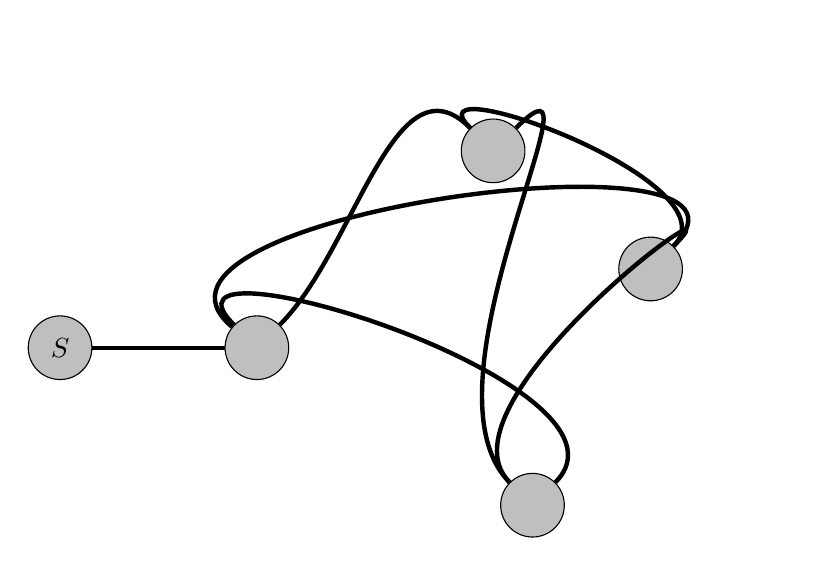
\begin{tikzpicture}[scale = 0.5]
\tikzset{vertex/.style = {shape=circle, draw, fill=gray!50, minimum size=2.3em}}
    \tikzset{edge/.style = {draw=green, ultra thick, -}}
% Define the coordinates of the start and end points of the edge
\node[vertex] (A) at (-5,0){$S$};
\node[vertex] (0) at (0,0){};
\node[vertex] (1) at (6,5){};
\node[vertex] (2) at (7,-4){};
\node[vertex] (3) at (10,2){};
\coordinate (end) at (2,2);

% Draw the circular edge
\draw[black, ultra thick] (0) to[out=45, in=135] (1);
\draw[black, ultra thick] (1) to[out=45, in=135] (2);
\draw[black, ultra thick] (2) to[out=45, in=135] (0);
\draw[black, ultra thick] (3) to[out=45, in=140] (0);
\draw[black, ultra thick] (3) to[out=45, in=135] (1);
\draw[black, ultra thick] (3) to[out=45, in=135] (2);
\draw[black, ultra thick] (A) to (0);


    
\end{tikzpicture} 
\end{frame}


\begin{frame}{TSP with Dynamic Programming(using Bitmask)}
   \centering
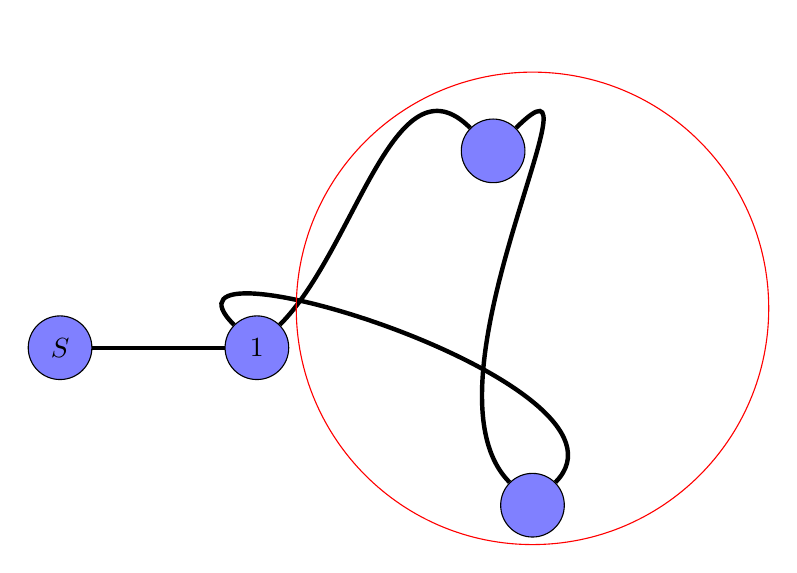
\begin{tikzpicture}[scale = 0.5]
\tikzset{vertex/.style = {shape=circle, draw, fill=blue!50, minimum size=2.3em}}
    \tikzset{edge/.style = {draw=green, ultra thick, -}}
% Define the coordinates of the start and end points of the edge
\node[vertex] (A) at (-5,0){$S$};
\node[vertex] (0) at (0,0){$1$};
\node[vertex] (1) at (6,5){};
\node[vertex] (2) at (7,-4){};
\coordinate (end) at (2,2);

% Draw the circular edge
\draw[black, ultra thick] (0) to[out=45, in=135] (1);
\draw[black, ultra thick] (1) to[out=45, in=135] (2);
\draw[black, ultra thick] (2) to[out=45, in=135] (0);
\draw[black, ultra thick] (A) to (0);

\draw [red](7,1) circle [radius=6cm];
    
\end{tikzpicture} 

\end{frame}
\begin{frame}{TSP with Dynamic Programming(using Bitmask)}
   \centering
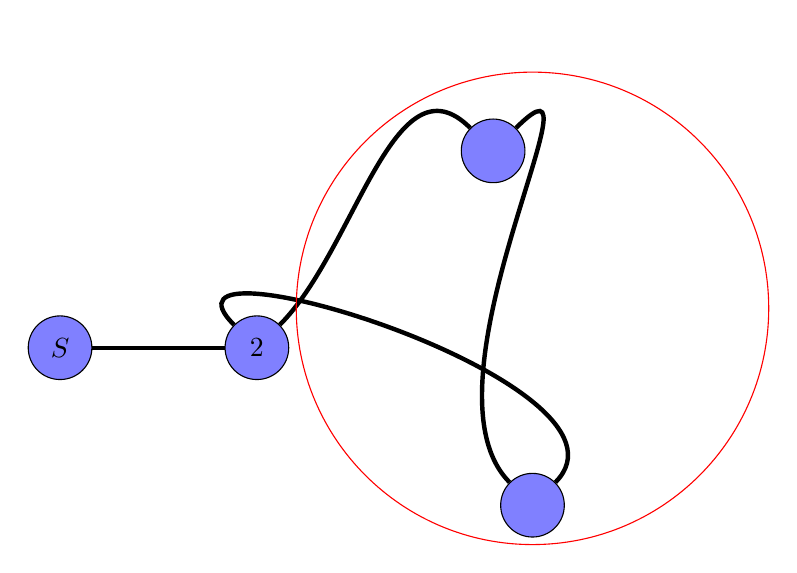
\begin{tikzpicture}[scale = 0.5]
\tikzset{vertex/.style = {shape=circle, draw, fill=blue!50, minimum size=2.3em}}
    \tikzset{edge/.style = {draw=green, ultra thick, -}}
% Define the coordinates of the start and end points of the edge
\node[vertex] (A) at (-5,0){$S$};
\node[vertex] (0) at (0,0){$2$};
\node[vertex] (1) at (6,5){};
\node[vertex] (2) at (7,-4){};
\coordinate (end) at (2,2);

% Draw the circular edge
\draw[black, ultra thick] (0) to[out=45, in=135] (1);
\draw[black, ultra thick] (1) to[out=45, in=135] (2);
\draw[black, ultra thick] (2) to[out=45, in=135] (0);
\draw[black, ultra thick] (A) to (0);
\draw [red](7,1) circle [radius=6cm];
\end{tikzpicture} 
\end{frame}




\begin{frame}{TSP with Dynamic Programming(using Bitmask)}
  \centering
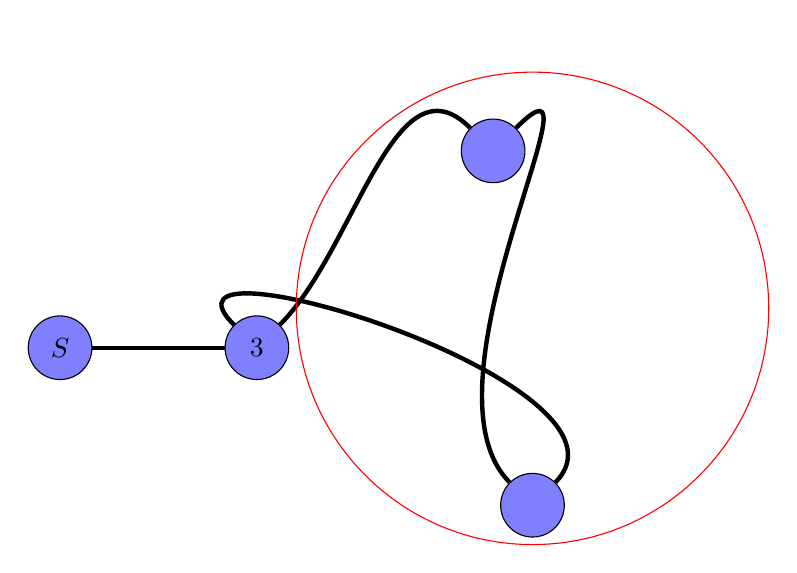
\begin{tikzpicture}[scale = 0.5]
\tikzset{vertex/.style = {shape=circle, draw, fill=blue!50, minimum size=2.3em}}
    \tikzset{edge/.style = {draw=green, ultra thick, -}}
% Define the coordinates of the start and end points of the edge
\node[vertex] (A) at (-5,0){$S$};
\node[vertex] (0) at (0,0){$3$};
\node[vertex] (1) at (6,5){};
\node[vertex] (2) at (7,-4){};
\coordinate (end) at (2,2);

% Draw the circular edge
\draw[black, ultra thick] (0) to[out=45, in=135] (1);
\draw[black, ultra thick] (1) to[out=45, in=135] (2);
\draw[black, ultra thick] (2) to[out=45, in=135] (0);
\draw[black, ultra thick] (A) to (0);
\draw [red](7,1) circle [radius=6cm];
\end{tikzpicture}  
\end{frame}
\begin{frame}{TSP with Dynamic Programming(using Bitmask)}
   \newtheorem{Which path should we choose?}{Which path should we choose?}
\begin{Which path should we choose?}
 We will choose the node so that $distance[S][i] + Cost_{remaining}$ becomes minimum
\end{Which path should we choose?}
   \newtheorem{Our Concern!!!}{Our Concern!!!}
\begin{Our Concern!!!}
 How to find the optimal path from remaining portion? 
\end{Our Concern!!!}
\begin{figure}
     \centering
     \includegraphics[scale=0.3]{Screenshot 2024-02-20 052919.png}
     \label{fig:enter-label}
 \end{figure}
  
\end{frame}
\begin{frame}{TSP with Dynamic Programming(using Bitmask)}
\begin{figure}
    \centering
    \includegraphics[scale=0.2]{Screenshot 2024-02-20 053629.png}
    
    \label{fig:enter-label}
\end{figure}
\newtheorem{Solution}{Solution}
\begin{Solution}
    \textbf{Here Comes \textcolor{red}{Recursion!}}
    \begin{figure}
        \centering
        \includegraphics[scale = 0.6]{Screen-Shot-2020-04-23-at-10.17.36-PM.png}
        \label{fig:enter-label}\cite{shafaetsplanet-dp}
    \end{figure}
\end{Solution}    

\end{frame}
\begin{frame}{TSP with Dynamic Programming(using Bitmask)}
        \newtheorem{Steps to perform Dynamic Programming(using Bitmask)}{Steps to perform Dynamic Programming(using Bitmask)}
\begin{Steps to perform Dynamic Programming(using Bitmask)}
  \begin{itemize}
      \item Initialize a DP table to store the optimal solution for subproblems. The DP table can be a 2D array where dp[mask][i] represents the minimum cost of visiting all vertices in the subset represented by the bitmask mask and ending at vertex i.
      \item Initialize the DP table for the base case where only one vertex is visited (i.e., dp[1 << i][i] = 0 for all vertices i).
      \item terate over all possible subsets of vertices represented by bitmasks and all possible ending vertices. For each subset and ending vertex, compute the optimal cost based on the previously computed values.
      \item he final answer will be the minimum value among all values dp[(1 << n) - 1][i], where i varies from 0 to n-1
  \end{itemize}
\end{Steps to perform Dynamic Programming(using Bitmask)}
\end{frame}


\begin{frame}{Time Complexity}
\newtheorem{Time Complexity}{Time Complexity}
\begin{Time Complexity}
$O(n^2 \cdot 2^n)$ where $O(n \cdot 2^n)$ are maximum number of unique subproblems/states and O(n) for transition (through for loop as in code) in every states.
\end{Time Complexity}
\end{frame}

% Jayed's Part ended


% Iffat's Part started

\subsection{TSP with Approximation Algorithm}
\begin{frame}{TSP with Approximation Algorithm}
\section*{What is Approximation Algorithm}
\newtheorem{Approximation Algorithm}{Approximation Algorithm}
\begin{Approximation Algorithm}
    \begin{itemize}
    \item  An approximation algorithm is a way of dealing with NP-completeness for an optimization problem. 
    \item This technique does not guarantee the best solution.
    \item The approximate algorithms work only if the problem instance satisfies \textbf{\textcolor{red}{Triangle-Inequality}. }
\end{itemize}
\end{Approximation Algorithm}   
\end{frame}
\begin{frame}{TSP with Approximation Algorithm}
\newtheorem{Triangle-Inequality}{Triangle-Inequality}
\begin{Triangle-Inequality}
    The least distant path to reach a vertex j from i is always to reach j directly from i, rather than through some other vertex k (or vertices), i.e., dis(i, j) is always less than or equal to dis(i, k) + dist(k, j). \cite{geeksforgeeks-tsp-approx-mst}
    \end{Triangle-Inequality}
    \newtheorem{Why Triangle-Inequality is a necessary condition?}{Why Triangle-Inequality is a necessary condition?}
\begin{Why Triangle-Inequality is a necessary condition?}
    When the cost function satisfies the triangle inequality, we can design an approximate algorithm for TSP that returns a tour whose cost is never more than twice the cost of an optimal tour.
    \end{Why Triangle-Inequality is a necessary condition?}
\end{frame}

\begin{frame}{TSP with Approximation Algorithm}
    In the traveling salesperson problem, the optimization problem is to find the \textbf{shortest cycle}, and the approximation problem is to find a short cycle.\\
    \newtheorem{Steps to perform Approximation Algorithm}{Steps to perform Approximation Algorithm}
\begin{Steps to perform Approximation Algorithm}
    \begin{itemize}
    \item  Let any node as starting node of the given graph
    \item Construct MST from with starting node as root.\\
    Two ways to find MST\\
    \begin{itemize}
        \item Prim’s Algorithm
        \item Kruskal's Algorithm
    \end{itemize}
    \item List vertices visited in preorder walk(DFS) of the constructed MST and add starting node at the end.
\end{itemize}
\end{Steps to perform Approximation Algorithm}



\end{frame}
\begin{frame}{TSP with Approximation Algorithm}
Let's take an example.\\Consider A as starting node\\
\begin{example}
  \centering
        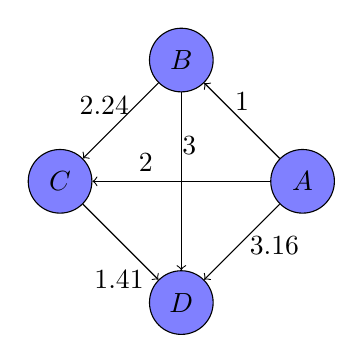
\begin{tikzpicture}[scale=0.22]
    \tikzset{vertex/.style = {shape=circle, draw, fill=blue!50, minimum size=2.3 em}}
    \tikzset{edge/.style = {draw=green, ultra thick, -}}

    % vertices
    \node[vertex] (b) at  (7,0) {$A$};
    \node[vertex] (c) at  (0,7) {$B$};
    \node[vertex] (d) at  (-7,0){$C$};
    \node[vertex] (e) at  (0,-7){$D$};

    % edges
    \draw [->] (b) -- node[pos = 0.8, above,xshift = 7mm]{3.16} (e);
    \draw [->] (b) -- node[midway, above]{1} (c);
    \draw [->] (b) -- node[pos=0.7,above]{2} (d);
    \draw [->] (c) -- node[pos= 0.3pt,xshift = 1mm]{3} (e);
    \draw [->] (c) -- node[pos= 0.3pt,xshift = -4mm]{2.24} (d);
    \draw [->] (d) -- node[pos=1, xshift = -5mm]{1.41} (e);
\end{tikzpicture}
\end{example}
\end{frame}



\begin{frame}{TSP with Approximation Algorithm}
  \centering
        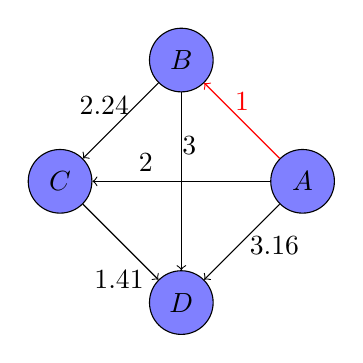
\begin{tikzpicture}[scale=0.22]
    \tikzset{vertex/.style = {shape=circle, draw, fill=blue!50, minimum size=2.3 em}}
    \tikzset{edge/.style = {draw=green, ultra thick, -}}

    % vertices
    \node[vertex] (b) at  (7,0) {$A$};
    \node[vertex] (c) at  (0,7) {$B$};
    \node[vertex] (d) at  (-7,0){$C$};
    \node[vertex] (e) at  (0,-7){$D$};

    % edges
    \draw [->] (b) -- node[pos = 0.8, above,xshift = 7mm]{3.16} (e);
    \draw [->,red] (b) -- node[midway, above]{1} (c);
    \draw [->] (b) -- node[pos=0.7,above]{2} (d);
    \draw [->] (c) -- node[pos= 0.3pt,xshift = 1mm]{3} (e);
    \draw [->] (c) -- node[pos= 0.3pt,xshift = -4mm]{2.24} (d);
    \draw [->] (d) -- node[pos=1, xshift = -5mm]{1.41} (e);
\end{tikzpicture}
\\
\\
Caption: Constructing MST
\end{frame}
\begin{frame}{TSP with Approximation Algorithm}
  \centering
        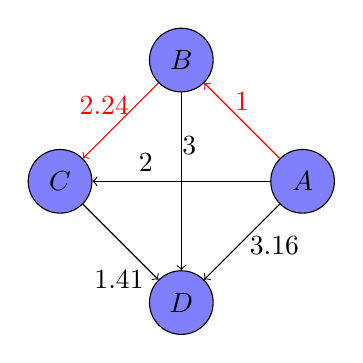
\begin{tikzpicture}[scale=0.22]
    \tikzset{vertex/.style = {shape=circle, draw, fill=blue!50, minimum size=2.3 em}}
    \tikzset{edge/.style = {draw=green, ultra thick, -}}

    % vertices
    \node[vertex] (b) at  (7,0) {$A$};
    \node[vertex] (c) at  (0,7) {$B$};
    \node[vertex] (d) at  (-7,0){$C$};
    \node[vertex] (e) at  (0,-7){$D$};

    % edges
    \draw [->] (b) -- node[pos = 0.8, above,xshift = 7mm]{3.16} (e);
    \draw [->,red] (b) -- node[midway, above]{1} (c);
    \draw [->] (b) -- node[pos=0.7,above]{2} (d);
    \draw [->] (c) -- node[pos= 0.3pt,xshift = 1mm]{3} (e);
    \draw [->,red] (c) -- node[pos= 0.3pt,xshift = -4mm]{2.24} (d);
    \draw [->] (d) -- node[pos=1, xshift = -5mm]{1.41} (e);
\end{tikzpicture}
\\
\\
Caption: Constructing MST
\end{frame}
\begin{frame}{TSP with Approximation Algorithm}
  \centering
        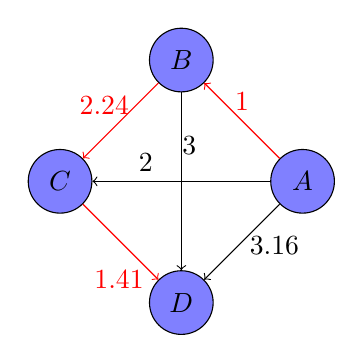
\begin{tikzpicture}[scale=0.22]
    \tikzset{vertex/.style = {shape=circle, draw, fill=blue!50, minimum size=2.3 em}}
    \tikzset{edge/.style = {draw=green, ultra thick, -}}

    % vertices
    \node[vertex] (b) at  (7,0) {$A$};
    \node[vertex] (c) at  (0,7) {$B$};
    \node[vertex] (d) at  (-7,0){$C$};
    \node[vertex] (e) at  (0,-7){$D$};

    % edges
    \draw [->] (b) -- node[pos = 0.8, above,xshift = 7mm]{3.16} (e);
    \draw [->,red] (b) -- node[midway, above]{1} (c);
    \draw [->] (b) -- node[pos=0.7,above]{2} (d);
    \draw [->] (c) -- node[pos= 0.3pt,xshift = 1mm]{3} (e);
    \draw [->,red] (c) -- node[pos= 0.3pt,xshift = -4mm]{2.24} (d);
    \draw [->,red] (d) -- node[pos=1, xshift = -5mm]{1.41} (e);
\end{tikzpicture}
\\
\\
Caption: Constructing MST
\end{frame}
\begin{frame}{TSP with Approximation Algorithm}
  \centering
        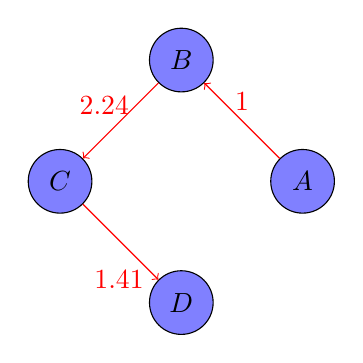
\begin{tikzpicture}[scale=0.22]
    \tikzset{vertex/.style = {shape=circle, draw, fill=blue!50, minimum size=2.3 em}}
    \tikzset{edge/.style = {draw=green, ultra thick, -}}

    % vertices
    \node[vertex] (b) at  (7,0) {$A$};
    \node[vertex] (c) at  (0,7) {$B$};
    \node[vertex] (d) at  (-7,0){$C$};
    \node[vertex] (e) at  (0,-7){$D$};

    % edges
    \draw [->,red] (b) -- node[midway, above]{1} (c);
    \draw [->,red] (c) -- node[pos= 0.3pt,xshift = -4mm]{2.24} (d);
    \draw [->,red] (d) -- node[pos=1, xshift = -5mm]{1.41} (e);
\end{tikzpicture}
\\
\\
Caption: Final MST
\end{frame}



\begin{frame}{TSP with Approximation Algorithm}
Now Perform DFS traversal on generated MST
\newtheorem{DFS traversal}{DFS traversal}
\begin{DFS traversal}

  \centering
    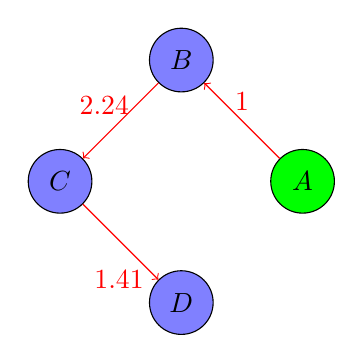
\begin{tikzpicture}[scale=0.22]
    \tikzset{vertex/.style = {shape=circle, draw, fill=blue!50, minimum size=2.3 em}}
    \tikzset{edge/.style = {draw=green, ultra thick, -}}

    % vertices
    \node[vertex,fill=green] (b) at  (7,0) {$A$};
    \node[vertex] (c) at  (0,7) {$B$};
    \node[vertex] (d) at  (-7,0){$C$};
    \node[vertex] (e) at  (0,-7){$D$};

    % edges
    \draw [->,red] (b) -- node[midway, above]{1} (c);
    \draw [->,red] (c) -- node[pos= 0.3pt,xshift = -4mm]{2.24} (d);
    \draw [->,red] (d) -- node[pos=1, xshift = -5mm]{1.41} (e);
\end{tikzpicture}
\end{DFS traversal}
\end{frame}
\begin{frame}{TSP with Approximation Algorithm}
MST under
\newtheorem{DFS traversal}{DFS traversal}
\begin{DFS traversal}

  \centering
    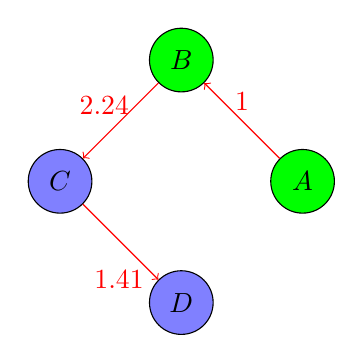
\begin{tikzpicture}[scale=0.22]
    \tikzset{vertex/.style = {shape=circle, draw, fill=blue!50, minimum size=2.3 em}}
    \tikzset{edge/.style = {draw=green, ultra thick, -}}

    % vertices
    \node[vertex,fill=green] (b) at  (7,0) {$A$};
    \node[vertex,fill=green] (c) at  (0,7) {$B$};
    \node[vertex] (d) at  (-7,0){$C$};
    \node[vertex] (e) at  (0,-7){$D$};

    % edges
    \draw [->,red] (b) -- node[midway, above]{1} (c);
    \draw [->,red] (c) -- node[pos= 0.3pt,xshift = -4mm]{2.24} (d);
    \draw [->,red] (d) -- node[pos=1, xshift = -5mm]{1.41} (e);
\end{tikzpicture}
\end{DFS traversal}
\end{frame}
\begin{frame}{TSP with Approximation Algorithm}
MST under 
\newtheorem{DFS traversal}{DFS traversal}
\begin{DFS traversal}

  \centering
    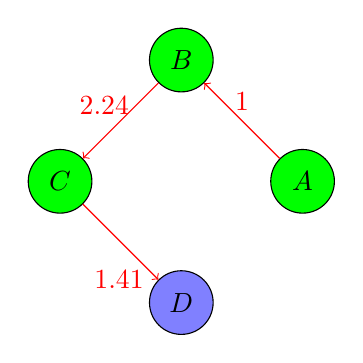
\begin{tikzpicture}[scale=0.22]
    \tikzset{vertex/.style = {shape=circle, draw, fill=blue!50, minimum size=2.3 em}}
    \tikzset{edge/.style = {draw=green, ultra thick, -}}

    % vertices
    \node[vertex,fill=green] (b) at  (7,0) {$A$};
    \node[vertex,fill=green] (c) at  (0,7) {$B$};
    \node[vertex,fill=green] (d) at  (-7,0){$C$};
    \node[vertex] (e) at  (0,-7){$D$};

    % edges
    \draw [->,red] (b) -- node[midway, above]{1} (c);
    \draw [->,red] (c) -- node[pos= 0.3pt,xshift = -4mm]{2.24} (d);
    \draw [->,red] (d) -- node[pos=1, xshift = -5mm]{1.41} (e);
\end{tikzpicture}
\end{DFS traversal}
\end{frame}
\begin{frame}{TSP with Approximation Algorithm}
MST under
\newtheorem{DFS traversal}{DFS traversal}
\begin{DFS traversal}

  \centering
    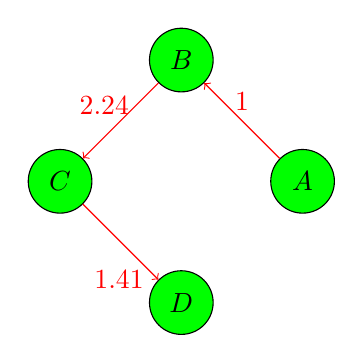
\begin{tikzpicture}[scale=0.22]
    \tikzset{vertex/.style = {shape=circle, draw, fill=blue!50, minimum size=2.3 em}}
    \tikzset{edge/.style = {draw=green, ultra thick, -}}

    % vertices
    \node[vertex,fill=green] (b) at  (7,0) {$A$};
    \node[vertex,fill=green] (c) at  (0,7) {$B$};
    \node[vertex,fill=green] (d) at  (-7,0){$C$};
    \node[vertex,fill=green] (e) at  (0,-7){$D$};

    % edges
    \draw [->,red] (b) -- node[midway, above]{1} (c);
    \draw [->,red] (c) -- node[pos= 0.3pt,xshift = -4mm]{2.24} (d);
    \draw [->,red] (d) -- node[pos=1, xshift = -5mm]{1.41} (e);
\end{tikzpicture}
\end{DFS traversal}
The full walk of above tree A \rightarrow B \rightarrow C \rightarrow D\\
$Cost_{\text{MST}} = Weight_{AB} + Weight_{BC} + Weight_{CD}$\\
\hspace{40}=$1+2.24+1.41$\\
\hspace{40}=$4.65$
\end{frame}
\begin{frame}{TSP with Approximation Algorithm}
\newtheorem{Facts}{Facts}
\begin{Facts}
\begin{itemize}
    \item $Cost_{\text{Best possible Travelling Salesman tour}} \geq Cost_{\text{MST}}$.
    \item The definition of MST says, it is a minimum cost tree that connects all vertices.
    \item $Cost_{\text{Best possible Travelling Salesman tour}} \leq 2 \cdot Cost_{\text{MST}}$.
    \item Every edge of MST is visited at most twice.
\end{itemize}
\end{Facts}
\end{frame}


\begin{frame}{TSP with Approximation Algorithm}
\newtheorem{Time Complexity}{Time Complexity}
\begin{Time Complexity}
Overall time complexity is dominated by the MST construction step, which is typically O(E log V) 
\end{Time Complexity}
\end{frame}
\section{Comparison between Exact and Approximate Solution}
\begin{frame}{Comparison between Exact and Approximate Solution}
    \newtheorem{Exact solution from DP}{Exact solution from DP}
    \begin{Exact solution from DP}
    $Result_{DP}=4.65$
    \end{Exact solution from DP}
    \newtheorem{Approximate solution from AA}{Approximate solution from AA}
    \begin{Approximate solution from AA}
    $Result_{AA}=2 \cdot Cost_{\text{MST}}=9.3$
    \end{Approximate solution from AA}
    \newtheorem{Ratio of two Sol^n}{Ratio  of two Sol^n}
    \begin{Ratio of two Sol^n}
    $Ratio=\frac{Result_{AA}}{Result_{DP}}=2$
    \end{Ratio of two Sol^n}
\end{frame}

% Iffat's Part ended



\bibliographystyle{plain}
\bibliography{ref}
\section{The End}
\begin{frame}{THE END}
   \begin{figure}
       \centering
       \includegraphics[scale=0.5]{Screenshot 2024-02-20 064258.png}
       
   \end{figure}
\end{frame}




\end{document}
